\chapter{Datasets}\label{Chapter:datasets}

\section{Lookup Tables}

\section{Symbol Rewriting}

\section{Micro Tasks}

CommAI mini tasks \citep{Baroni2017} are a set of strictly local and locally testable (please refer to section \ref{flt:sh}) languages designed to test the generalization capabilities of a compositional learner. Based on the mini tasks we propose a new dataset of sub-regular languages which we call he Micro Tasks. The language encompasses a vocabulary of all printable ascii characters, except printable but invisible characters i.e. tab, space, newline etc. 
\begin{itemize}
	\item Define verification and production tasks
	\item The vocabulary is acted upon by the boolean operators (or, and and not) in the case of both verification and production tasks. In case of verification we have an additional operation copy.
	\item Describe as in CommAI how copy and or are strictly local while and+not constitute locally k testable languages.
\end{itemize}


While the CommAI mini task position themselves as strictly local and locally testable tasks of progressive difficulty we add another layer of difficulty to the tasks by setting them up as either a decision problem(verify) or search problem(produce) in the same training domain.

\begin{figure}[ht] 
	\begin{subfigure}[b]{0.5\linewidth}
		\centering
		\ifpdf
		\includegraphics[width=0.95\linewidth]{./figs/micro/train_verify-pdf}
		\else
		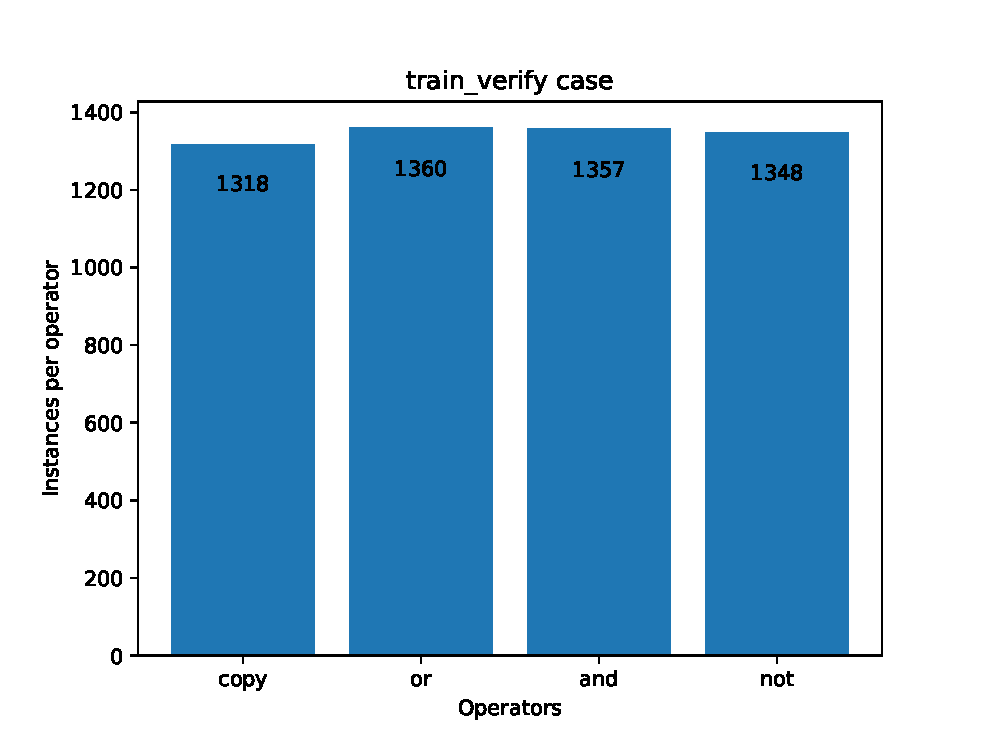
\includegraphics[width=0.95\linewidth]{./figs/micro/train_verify-eps}
		\fi
		\caption{Verification Task} 
		\label{tr_ver} 
		\vspace{4ex}
	\end{subfigure}%% 
	\begin{subfigure}[b]{0.5\linewidth}
		\centering
		\ifpdf
		\includegraphics[width=0.95\linewidth]{./figs/micro/train_produce-pdf}
		\else
		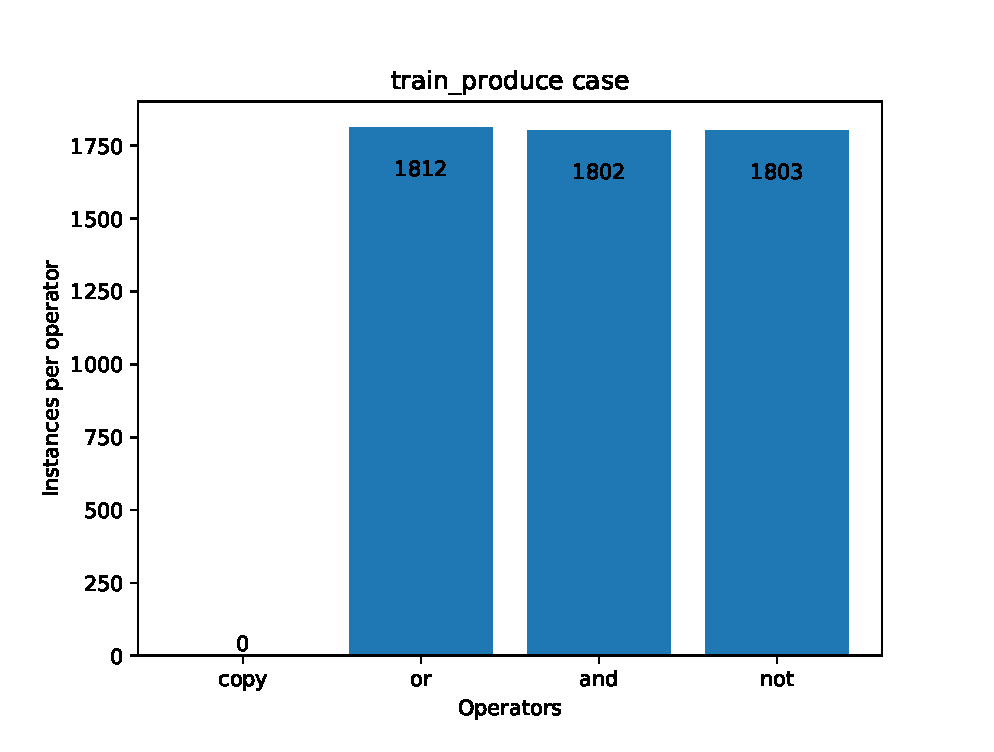
\includegraphics[width=0.95\linewidth]{./figs/micro/train_produce-eps}
		\fi 
		\caption{Production Task} 
		\label{tr_prd} 
		\vspace{4ex}
	\end{subfigure}
	\caption{Micro Tasks - Training Data}
	\label{micro_train}
\end{figure}

\begin{figure}[ht] 
	\begin{subfigure}[b]{0.5\linewidth}
		\centering
		\ifpdf
		\includegraphics[width=0.95\linewidth]{./figs/micro/unseen_verify-pdf}
		\else
		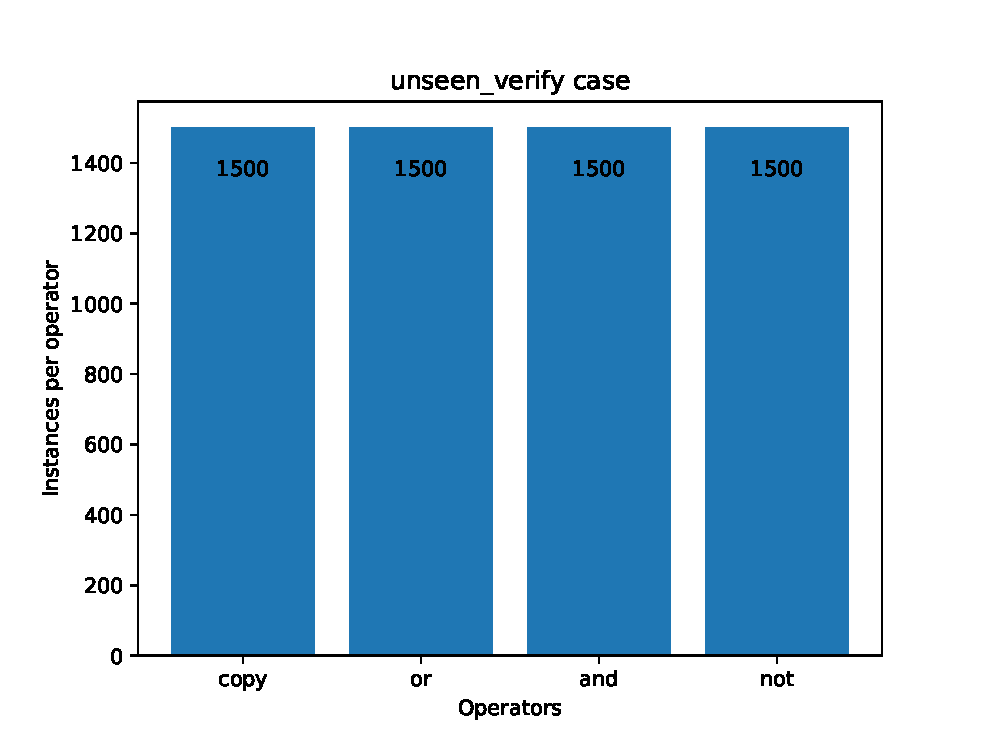
\includegraphics[width=0.95\linewidth]{./figs/micro/unseen_verify-eps}
		\fi
		\caption{Verification Task} 
		\label{un_ver} 
		\vspace{4ex}
	\end{subfigure}%% 
	\begin{subfigure}[b]{0.5\linewidth}
		\centering
		\ifpdf
		\includegraphics[width=0.95\linewidth]{./figs/micro/unseen_produce-pdf}
		\else
		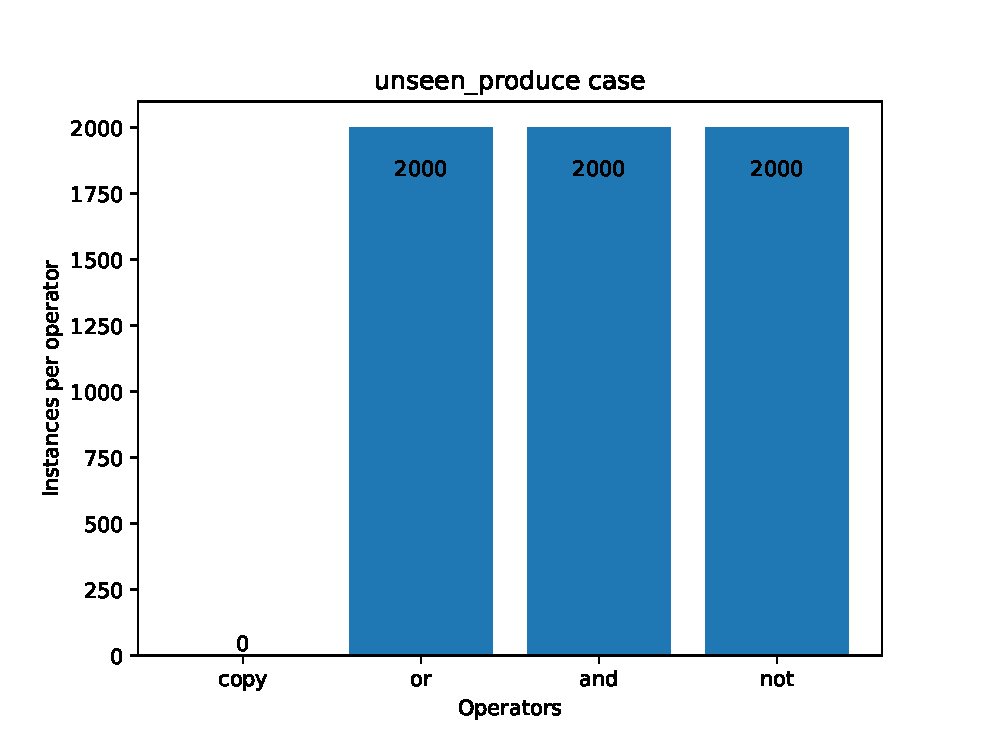
\includegraphics[width=0.95\linewidth]{./figs/micro/unseen_produce-eps}
		\fi 
		\caption{Production Task} 
		\label{un_prd} 
		\vspace{4ex}
	\end{subfigure}
	\caption{Micro Tasks - Unseen Data}
	\label{micro_test}
\end{figure}